\section{Framework}
\label{sec:framework_short_desc}
This project involves processing a large amount of data, requires a lot of compute power and working as a team with heterogeneous environments. Since we had anticipated that we'd be making a lot of experiments, we carefully designed a framework which allows training and keep a record of all experiments (reproducible code). All explanations on the framework we developed have been listed in appendix \ref{sec:training_fwk} . As a matter of fact, getting an accurate system was more of a software engineering challenge rather than a pure machine learning exploration. Our code is available on ~\href{https://github.com/balthazarneveu/molecule-retrieval-using-nlp}{GitHub} for future research.

\section{Our work}

\subsection*{Base model}
Figure \ref{fig:original_pipeline} depicts the approach we're taking: Text descriptions are transformed into sequences of tokens of various lengths (sequences of integers). Tokenized sequences are then embedded into a vector space using a large language model encoder.
Each description $T_{i}$ is transformed into a vector $t_{i}$ (text descriptions embeddings). 

Molecules $M_{i}$ will be transformed into vector descriptors $m_{i}$ (molecule embeddings). Each atom is first transformed into a vector using its neighboring atoms. The graph structure is kept as an undirected graphs to model the bounds between atoms. A graph convolutional network (GCN) is then used to embed these graphs into a vector space. The molecule and text descriptions embeddings are then compared. 

\textit{Contrastive learning is used to train such a model}: supervision comes from the knowledge of the pairing between the molecule and its text description. We compute a pairwise similarity between the molecule embedding $m_{i}$ and text embeddings $t_{i}$. The idea behind contrastive learning relies on maximizing similarity between molecules and text embeddings for the correct pair and minimized for the wrong pairs.

\textit{At inference time}, a chemist will query the system with a text sentence $T$ to search the database. The sentence query will be embedded into a vector $t$ which is compared to all molecules embeddings in a database. The most relevant molecules (highest similarity score) can be proposed to the chemist.

\subsection*{Preliminary study}
\label{sec:preliminary study}

\begin{table*}[ht]
    \centering
    \begin{tabular}{|c|c|c|c|c|}
    \hline
    \textbf{Experiment ID} & \textbf{Model Size} & \textbf{LLM} & \textbf{GNN} & \textbf{LRAP} \\ \hline
    101         & 593k                & Frozen Distill-Bert           & Base 3 layer GCN       & 18.7\%      \\ \hline
    106         & 964k                & Frozen Distill-Bert + Adapter & Base 3 layer GCN       & 26.8\%      \\ \hline
    114         & 2.125M              & Frozen Distill-Bert + Adapter & Big 5 layer GCN        & 31.6\%      \\ \hline
    112         & 964k                & Frozen Sci-Bert + Adapter     & Base 3 layer GCN       & 36.7\%      \\ \hline
    113         & 2.125M              & Frozen Sci-Bert + Adapter     & Big 5 layer GCN        & 39.8\%      \\ \hline
    65          & 66.9M               & Trainable Bert                & Base 3 layer GCN       & 63.5\%      \\ \hline
    400         & 110M                & Trainable Sci-Bert            & Base 3 layer GCN       & 66\%        \\ \hline
    \end{tabular}
    \caption{Base Models Specifications and Performances}
    \label{tab:preliminary_study_metrics}
\end{table*}


We start with a few toy experiments to see which architecture factors are most promising (initial hope is that the performances will scale accordingly when we add all extra machine learning tricks).
\textbf{Frozen LLM weights}: We first started with by simple models based on the base GCN (3 graph convolution layers followed by a global pooling layer and 2 layers MLP). Instead of fine tuning all parameters of the LLM, we first started by freezing the LLM parameters. Although simple, this idea intuitively has many advantages for training:
\begin{itemize}
    \item We discard the huge memory cost of training a LLM (memory issues not only come from storing the weights on the GPU but all the optimizers variables during back propagation). The idea could have been pushed further by pre-computing the text embeddings and storing them on disk. 
    \item Intuitively, freezing the LLM parameters should make the training more stable as the LLM embeddings acts as a kind of anchor that the GNN shall match.
\end{itemize}
Unfortunately, training achieves low accuracy although the number of parameters to train is lightweight. We added an "adapter" module which is simply a MLP which will adapt by projecting the text representations into a more adapted space which can match with the graph.
\textbf{Influence of the graph neural network size}: We pursued our explorations to see the impact of the GNN size. The \textbf{big GCN} (5 graph convolution layers with 2 residual connection) is more complex and has more parameters to train. We can see that the accuracy is improved by increasing the GCN size. 
\begin{itemize}
    \item Using frozen Distil-BERT: from experiment 106 (base GCN $\text{LRAP}=26.8\%$) to 114 - (big GCN $\text{LRAP}=31.6\%$)
    \item Using frozen SciBERT: from experiment 102 (base GCN $\text{LRAP}=36.7\%$) to 113 - (big GCN $\text{LRAP}=39.8\%$)
\end{itemize}


\textbf{Influence of the pretrained language model}: We also browsed Hugging Face to find models that could be dedicated to scientific-specific language processing. We found the Sci-Bert\cite{scibert} model and could use it as a drop-in replacement for the Distil-Bert baseline model. Improvements were two-fold when changing the pretrained LLM during this preliminary study: a tokenizer dedicated to a scientific corpus seems by nature a natural choice for scientific words...here atoms and molecule names not being too frequent in common language. The Sci-Bert model may also have reasoning capabilities closer to science and chemistry reactions. This was translated by a improvement in performances. Increasing the GNN size improves accuracy.
\begin{itemize}
    \item Using the Base GCN : from experiment 106 Distil-BERT ($\text{LRAP}=26.8\%$) to experiment 112 - SciBert ($\text{LRAP}=36.7\%$).
    \item Using the Big-GCN: from experiment 114 Distil-BERT ($\text{LRAP}=31.6\%$) to experiment 113 - SciBert ($\text{LRAP}=39.8\%$).
\end{itemize}
The capacity of the network (same number of parameters) being fixed between these two experiments, it proves that the SciBERT tokenization and pretraining is definitely more suited for our task. We'd hope that this $seq 8\%$ LRAP improvement would be translated when training a fully trainable LLM.

Unfortunately we later conducted larger experiments with fully trainable LLM (starting from the pretrained weights) and the performances differences were not as good as expected. Using the Base GCN : from experiment 65 Distil-BERT ($\text{LRAP}=63.5\%$) to experiment 400 - SciBert ($\text{LRAP}=66\%$), there's not that $seq 8\%$ LRAP improvement that we had seen earlier. Furthermore, it's hard to tell whether the 2.5\% improvement is due to the SciBert model pretraining being more suited for our task or the fact that the model has nearly twice as many trainable parameters than the Distil-BERT. 

This preliminary study gave us guidance that using a larger GCN and using SciBERT pretrained weights and tokenizer were good trends to follow to try improving our results. The pitfall is that fine tuning SciBERT comes with a bigger memory footprint than Distil-BERT which requires diminishing batch sizes for a fixed GPU (and as stated in the CLIP paper, large batch size seems to be one key factor of the success of contrastive learning). Experiments 65 and 400 have been cautiously trained with batches of size 32 and same hyperparameters to get comparable results: 
\begin{itemize}
    \item the SciBERT experiment 400 was only possible using a NVIDIA RTX A4000 with 24Gb of RAM \item the Distil-BERT experiment 65 was possible on a NVIDIA Tesla T100 with 16Gb of RAM (Kaggle Kernels notebook).
\end{itemize}



\begin{figure*}[ht]
    \centering
    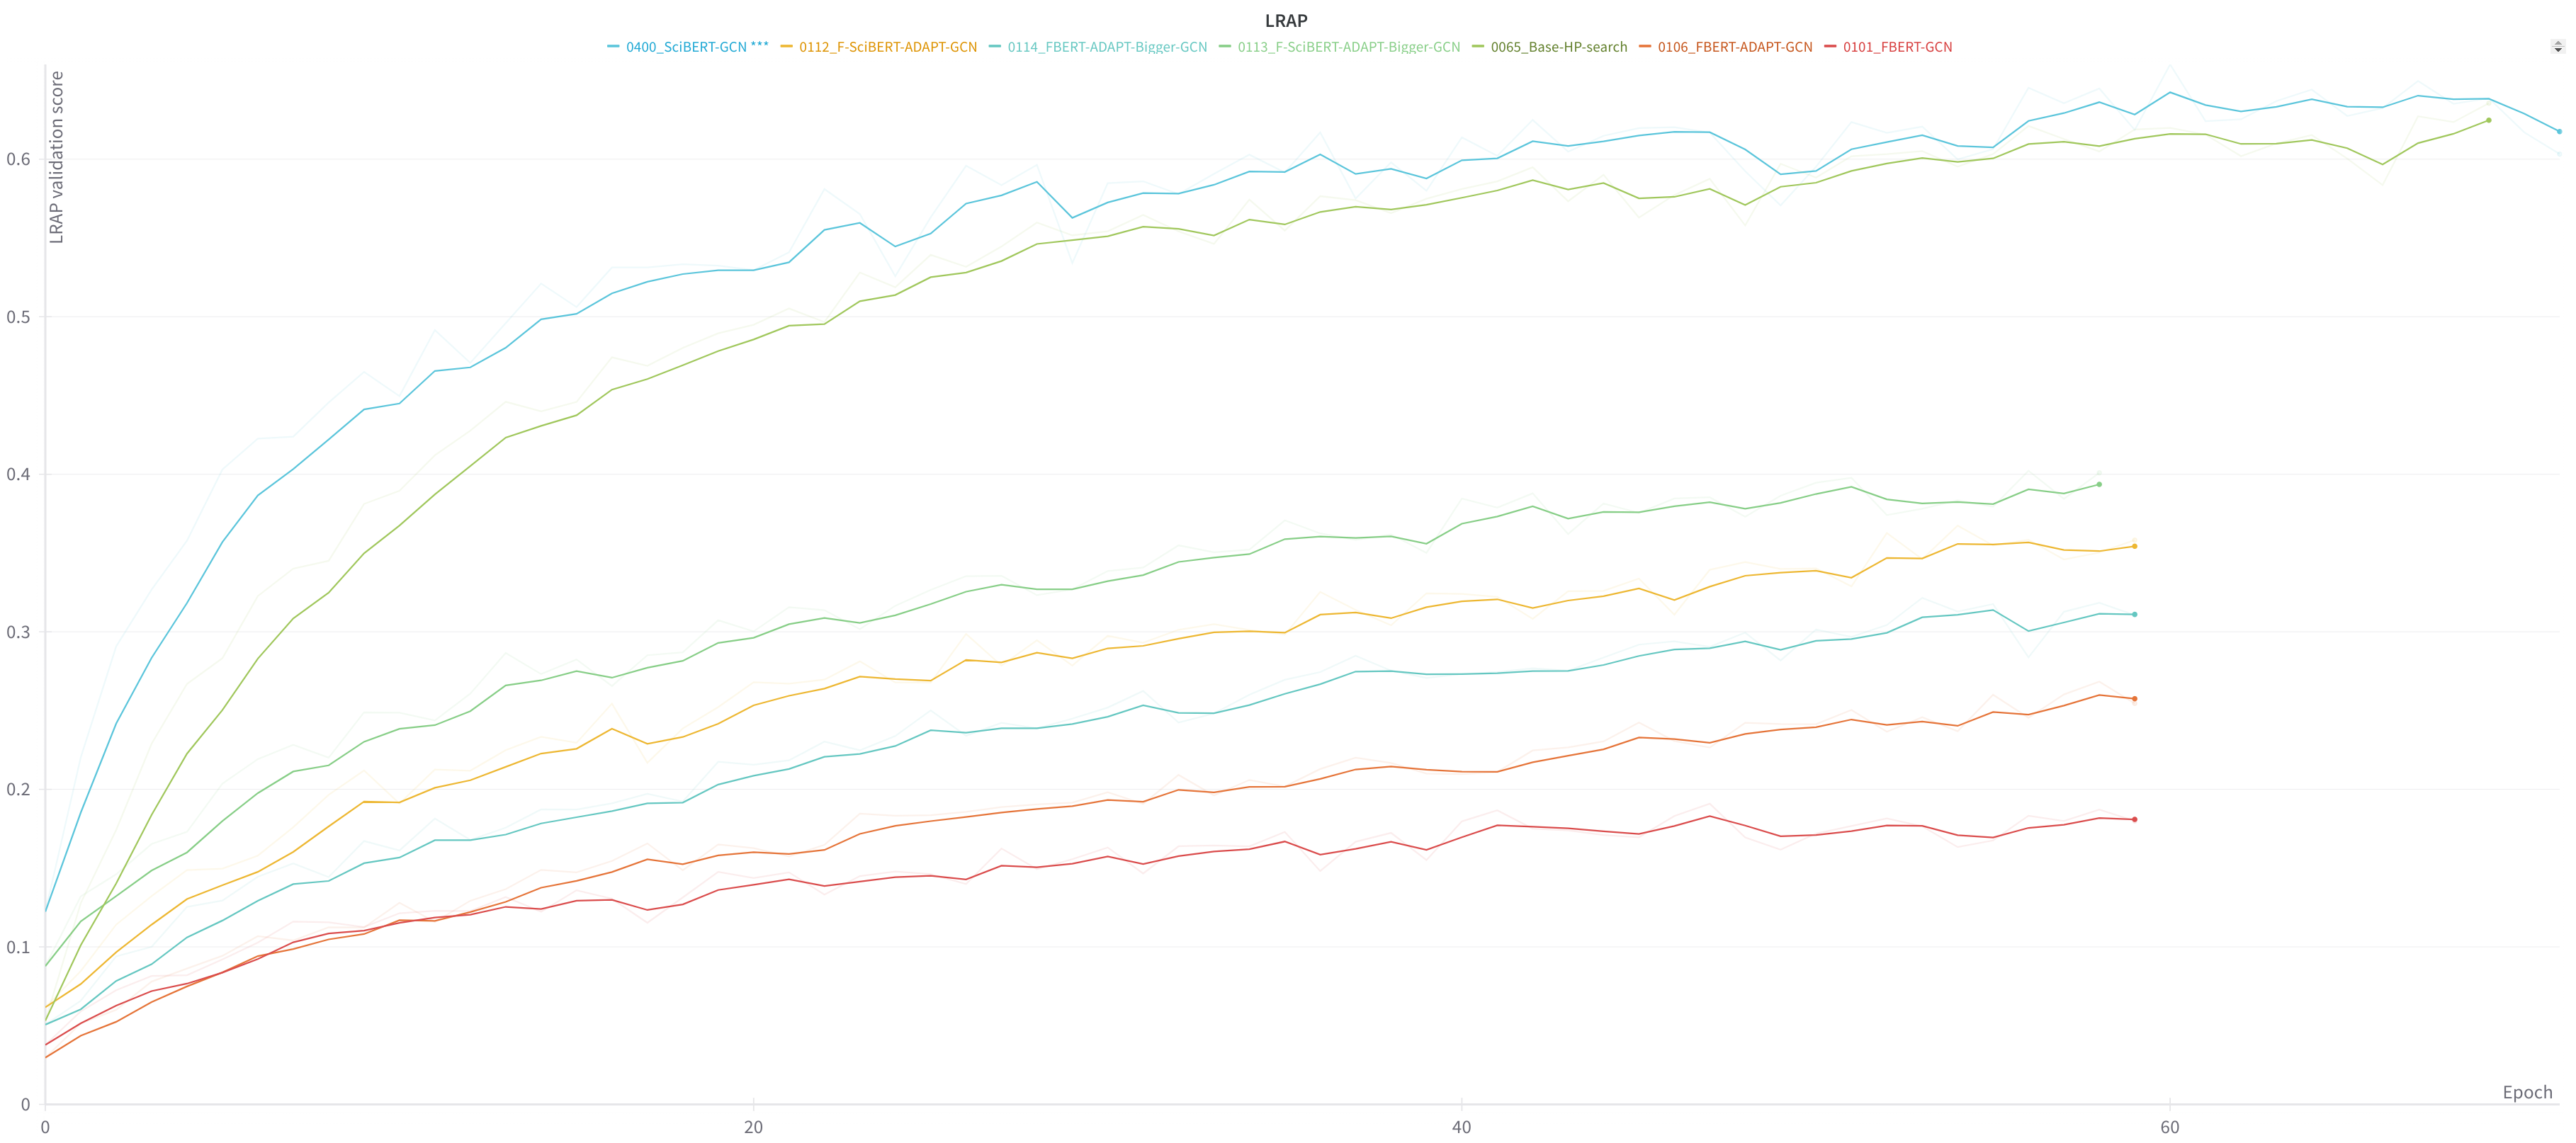
\includegraphics[width=1.\textwidth]{figures/preliminary_study.png}
    \caption{Training curves for the preliminary study.}
    \label{fig:preliminary_study_curves}
\end{figure*}



\subsection*{Our model}
\label{sec:our model}
We have trained and experimented with several models throughout this project. We identified axes which left room for improvement of the LRAP score and we tried to combine them to create the most robust and efficient model. We started from the baseline model and toyed with the hyperparameters (learning rate), altered the loss function, augmented the size of the GCN and 

\color{red}TODO - batch size, scheduler, hyperparameters, GPU memory occupancy, archi, LRAP \color{black}

\color{red}TODO - Training curves side by side with LR \color{black}

An ensembling technique is later used to average the scores of each model which leads to an extra accuracy improvement as suggested in \cite{text2mol}. (average submission csv for experiments 9008 and 9009 basically, a trick which has no extra cost and allows taking more confident desisions).